\documentclass{article}
\usepackage[margin=1in]{geometry}
\usepackage{forest}
\usepackage{tabu}
\usepackage{listings}
\usepackage{amsmath}
\usepackage{amsfonts}
\usepackage{float}
\usepackage{color}
\usepackage{multicol}
\usepackage[colorlinks = true,
            linkcolor = blue,
            urlcolor  = blue,
            citecolor = blue,
            anchorcolor = blue]{hyperref}
\usepackage{subfig}
\usepackage[font=small,labelfont=bf]{caption} % Required for specifying 
                                              % captions to tables and figures

\newcommand{\MYhref}[3][blue]{\href{#2}{\color{#1}{#3}}}%

\definecolor{dkgreen}{rgb}{0,0.6,0}
\definecolor{gray}{rgb}{0.5,0.5,0.5}
\definecolor{mauve}{rgb}{0.58,0,0.82}

\lstset{frame=tb,
  language=Java,
  aboveskip=3mm,
  belowskip=3mm,
  showstringspaces=false,
  columns=flexible,
  basicstyle={\small\ttfamily},
  numbers=none,
  numberstyle=\tiny\color{gray},
  keywordstyle=\color{blue},
  commentstyle=\color{dkgreen},
  stringstyle=\color{mauve},
  breaklines=true,
  breakatwhitespace=true,
  tabsize=3
}

\title{CPSC 524 Assignment 2: Area of the Mandelbrot Set}
\author{Rami Pellumbi\thanks{M.S., Statistics \& Data Science}}
\date{\today}

\begin{document}

\maketitle

\newpage 

\section{Introduction}

This assignment focuses on assessing the performance gains achievable through 
the application of loop directives and tasks in parallelizing the computation 
of the Mandelbrot set area. The basis for this study is a serial algorithm 
designed for this task, detailed as follows:

\begin{enumerate}
    \item We begin by defining a rectangular region in the complex plane, denoted as \textbf{R}. This region is bounded by the lower-left corner $-2.0 + 0.0i$ and the upper-right corner $0.5 + 1.25i$.
    \item This region \textbf{R} is then discretized into a grid of cells, each having a side length of 0.001 units. The set of all possible lower-left corner coordinates of these cells is represented by $T$, defined as:
    \begin{align*}
        T := \{(x, y) : x \in X, y \in Y \},
    \end{align*}
    where 
    \begin{align*}
        X &= \{x \in \mathbb{R} : x = -2.0 + n * 0.001, -2.0 \leq x < 0.5, n \in \mathbb{N}\}, \\
        Y &= \{y \in \mathbb{R} : y = 0.0 + n * 0.001, 0.0 \leq y < 1.25, n \in \mathbb{N}\}.
    \end{align*}
    A cell is uniquely defined by its lower-left corner coordinate $(x, y) \in X \times Y$. 
    We denote such a cell by $C_{x,y}$, and the set of all such cells is $C := \{C_{x, y}: (x, y) \in T\}$.
    
    A few clarifying remarks:
    \begin{itemize}
        \item The cardinality of $X$ is $$\lvert X \rvert = \frac{0.5 - (-2.0)}{0.001} = 2500.$$
        \item The cardinality of $Y$ is $$\lvert Y \rvert = \frac{1.25 - 0.0}{0.001} = 1250.$$
        \item The cardinality of $T$ is $$\lvert T \rvert = \lvert X \rvert \cdot \lvert Y \rvert = 2500 \cdot 1250 = 3125000.$$
    \end{itemize}
    
    \item For each cell $C_{x, y} \in C$, a random point $c$ within the cell is generated.
    \item The Mandelbrot update $z \leftarrow z^2 + c$ is iteratively computed for this random point $c$, for up to 25,000 iterations.
    \begin{enumerate}
        \item If the condition $\lvert z \rvert^2 > 4$ is met at any iteration, the point $c$ is marked as being outside the Mandelbrot set.
        \item Conversely, if all 25,000 iterations are completed without meeting this condition, the point $c$ is considered to be inside the Mandelbrot set.
    \end{enumerate}
    
    Let $N_I$ and $N_O$ denote the total number of points that are inside and outside the Mandelbrot set, respectively.
    \item The area estimate for the Mandelbrot set is computed as:
    \begin{align*}
        A = 2.0 \cdot \frac{N_I}{N_O + N_I} \cdot \text{Area}(\textbf{R}),
    \end{align*}
    where $\text{Area}(\textbf{R}) = 2.5 \times 1.25 = 3.125$.
\end{enumerate}

\section{Project Organization}

The project is laid out to provide a clean separation of source files, header files, compiled objects, and documentation. 

\begin{multicols}{2}
    \begin{forest}
        for tree={
            font=\ttfamily,
            grow'=0,
            child anchor=west,
            parent anchor=south,
            anchor=west,
            calign=first,
            edge path={
                \noexpand\path [draw, \forestoption{edge}]
                (!u.south west) +(7.5pt,0) |- node[fill,inner sep=1.25pt] {} (.child anchor)\forestoption{edge label};
            },
            before typesetting nodes={
                if n=1
                {insert before={[,phantom]}}
                {}
            },
            fit=band,
            before computing xy={l=15pt},
        }
    [a2
        [bin/]
        [docs/]
        [include/]
        [out/]
        [src/]
        [build-run-part1.sh]
        [build-run-part2.sh]
        [build-run-part3.sh]
        [build-run-part4.sh]
        [Makefile]
    ]
    \end{forest}
    \columnbreak
    \begin{itemize}
        \item \textbf{bin/}: The \texttt{bin} folder holds compiled objects and executable files, centralizing the output of the compilation process.
        \item \textbf{docs/}: This folder contains LaTeX files and other documentation materials that pertain to the report.
        \item \textbf{include/}: Here, all the header files (\texttt{.h}) are stored. These headers contain function prototypes and static inline functions used across different benchmarks.
        \item \textbf{out/}: The \texttt{out} folder stores the outputs from each task. Each subdirectory is of the relevant task. It also houses the csv files generated by the programs.
        \item \textbf{src/}: This directory houses the source files (\texttt{.c}) that make up the benchmarks.
        \item \textbf{Shell Scripts}: The shell scripts are at the root directory and are used to submit the job for the relevant task to slurm via \texttt{sbatch}. 
        \item \textbf{Makefile}: This Makefile has undergone extensive modifications to support the project hierarchy. It is engineered to handle the appropriate linking of shared libraries and integration of common code components, ensuring a seamless compilation process.
    \end{itemize}
\end{multicols}

\section{Code Explanation, Compilation, and Execution}

This section outlines the steps required to build and execute the code. The provided Bash scripts automate the entire process, 
making it straightforward to compile and run the code. All the below steps assume 
you are in the root of the project directory.

\subsection{Automated Building and Execution}
\begin{itemize}
    \item \textbf{Part 1: Serial Program} 
    There are two implementation of the serial program (to be elaborated in Section 4). 
    The command \texttt{sbatch build-run-part1.sh} will compile and run the files:
    \begin{itemize}
        \item \texttt{mandseq.c}: standard, slightly optimized, serial implementation of the algorithm.
        \item \texttt{mandseq-avx.c} more advanced implementation with AVX 512 instructions.
    \end{itemize}
    The output of the experiments will be in \texttt{out/serial.csv}.
    
    \item \textbf{Part 2: OMP Loop Directives}
    There are multiple programs run in Part 2. The programs associated with part 2 are:
    \begin{itemize}
        \item \texttt{mandomp.c}: extending \texttt{mandseq.c} to use OMP loop directives.
        \item \texttt{mandomp-avx.c}: extending \texttt{manseq-avx.c} to use OMP loop directives.
        \item \texttt{mandomp-ts.c}: a copy of \texttt{mandomp.c} using \texttt{drand-ts.c} for thread safe random number generation (RNG).
        \item \texttt{mandomp-ts-avx.c} a copy of \texttt{mandomp-avx.c} using \texttt{drand-ts.c} for thread safe RNG.
        \item \texttt{mandomp-collapse.c} a modification of \texttt{mandomp-ts.c} to support the collapse clause.
        \item \texttt{mandomp-collapse-avx.} a modification of \texttt{mandomp-ts-avx.c} to support the collapse clause.
    \end{itemize}
    The script \texttt{build-run-part2.sh} validates the weird behavior of the non thread safe RNG, shows how the fix 
    in \texttt{drand-ts.c} fixes the issue, and assesses the thread safe code against multiple thread counts and multiple 
    schedules. To run all the experiments, execute \texttt{sbatch build-run-part2.sh}. The results are stored in 
    \texttt{out/omp.csv}.

    \item \textbf{Part 3: OMP Tasks}
    In part 3, only the AVX version of the program is adopted to OMP Tasks. There are multiple programs run in Part 3. The programs associated with part 3 are:
    \begin{itemize}
        \item \texttt{mandomp-tasks.c}: extending \texttt{mandseq-avx.c} to use OMP tasks. One thread creates tasks and one task is created per batch of cells. 
        \item \texttt{mandomp-tasks-columns.c}: extending \texttt{mandomp-tasks.c} to instead create one task per column. One thread creates tasks.
        \item \texttt{mandomp-ts-columns-shared.c}: a copy of \texttt{mandomp-tasks-columns.c} but now all threads create tasks.
    \end{itemize}
    The script \texttt{build-run-part3.sh} assesses the area and wall clock time of the above progrmas. 
    To run all the experiments, execute \texttt{sbatch build-run-part3.sh}. The results are stored in \texttt{out/tasks.csv}.

    \item \textbf{Part 4: Parallel RNG}
    In part 4, \texttt{mandomp-ts-avx.c} is modified into \texttt{mandomp-ts-avx-parallel.c}. It makes use of the parallel random 
    number generator in \texttt{drand-ts.c}.
    To run all the experiments, execute \texttt{sbatch build-run-part4.sh}. The results are stored in \texttt{out/omp-parallel.csv}. 
\end{itemize}

\subsection{Post-Build Objects and Executables}
Upon successful compilation and linking, an \texttt{obj/} directory will be generated within the root directory. 
This directory will contain the compiled output files. Additionally, the executable files for running each part will be 
situated in the \texttt{bin/} directory.

\subsection{Output Files From \texttt{sbatch}}
The output files generated from running the code by submitting the relevant Bash script via \texttt{sbatch} will be 
stored in the relevant subdirectory of the \texttt{out} directory. 

\section{Serial Implementation}
\subsection{Standard and AVX}
The serial implementation was first written in the standard way to achieve a runtime of approximately 
49.2 seconds. After some searching, an optimized implementation using AVX 256 instructions was found.\footnote{Source: \MYhref{https://polarnick.com/blogs/other/cpu/gpu/sse/opencl/openmp/2016/10/01/mandelbrot-set-sse-opencl.html}{https://polarnick.com/blogs/other/cpu/gpu/sse/opencl/openmp/2016/10/01/mandelbrot-set-sse-opencl.html}} 
This source was rewritten to the assignment at hand using AVX 512 instructions found in the \MYhref{https://www.intel.com/content/www/us/en/docs/intrinsics-guide/index.html}{intel intrinsics guide}. 

\subsection{Standard Implementation}
\subsubsection{Implementation}
First, we iterate over the cells in \textbf{R} by a double for loop 
through the sets $X$ and $Y$. Concretely, the below loops iterate over all $(x, y) \in T$:
\newpage
\begin{lstlisting}
    for (size_t n = 0; n < 2500; n++)
    {
        double current_bottom_left_x = -2.0 + CELL_SIDE_LENGTH * n;
        for (size_t m = 0; m < 1250; m++)
        {
            double current_bottom_left_y = 0.0 + CELL_SIDE_LENGTH * m;
        }
    }
\end{lstlisting}
Next, for each cell, we generate a random coordinate inside the cell and perform the 
mandelbrot iteration on it. Since we are performing $N = 3125000$ iterations total, we 
can simply count the number of cells inside the mandelbrot set and then compute $N_O = N - N_I$. 
This gets rid of any conditional checks in the loop helping optimize.
Adjusting our for-loop above:
\begin{lstlisting}
    int N = 3125000, N_I = 0;
    for (size_t n = 0; n < 2500; n++)
    {
        double current_bottom_left_x = -2.0 + CELL_SIDE_LENGTH * n;
        double max_x = current_bottom_left_x + CELL_SIDE_LENGTH;
        for (size_t m = 0; m < 1250; m++)
        {
            double current_bottom_left_y = 0.0 + CELL_SIDE_LENGTH * m;
            double max_y = current_bottom_left_y + CELL_SIDE_LENGTH;
            // Get a random x and y inside of the cell
            double random_x = current_bottom_left_x + (max_x - current_bottom_left_x) * drand();
            double random_y = current_bottom_left_y + (max_y - current_bottom_left_y) * drand();
            // mandelbrot_iteration returns 0 if outside the set, else 1
            N_I +=  mandelbrot_iteration(random_x, random_y);
        }
    }
    int N_O = N - N_I; 
\end{lstlisting}
The \texttt{mandelbrot\_iteration} function checks if the complex number with real part 
\texttt{random\_x} and imaginary part \texttt{random\_y}. The implementation is 
found in \texttt{mandelbrot.h}. The function is static inlined to allow for portability 
between the multiple programs and is elaborated below:
\begin{lstlisting}
   static inline int mandelbrot_iteration(double c_re, double c_im, size_t max_iterations)
   {
       double z_re = 0.0, z_im = 0.0; // start at 0
       double magnitude_squared = 0.0;
   
       for (size_t i = 0; i < max_iterations; i++)
       {
           // compute the real part of z in the update
           double temp_re = z_re * z_re - z_im * z_im + c_re; 
           // compute the imaginary part of z in the update
           z_im = (z_re + z_re) * z_im + c_im; 
           z_re = temp_re;
           magnitude_squared = z_re * z_re + z_im * z_im;
           // break if we diverged
           if (magnitude_squared > 4.0) { return 0; }
       }
       return 1;
   } 
\end{lstlisting}
The update rule was done more optimally than just doing $z^2 + c$ via the pseudocode 
found in \MYhref{https://en.wikipedia.org/wiki/Mandelbrot_set}{Wikipedia}.
It is worth noting that complex numbers were manually handled via tracking two real numbers 
rather than using the \texttt{double complex} type from the \texttt{<complex.h>}. Using the complex 
library resulted in atrociously bad performance relative to using just doubles. This seems to 
be a \MYhref{https://stackoverflow.com/questions/42659668/stdcomplex-multiplication-is-extremely-slow}{a common issue}.

\subsubsection{Results}
Running the standard implementation 3 times, the following results were obtained:
\begin{table}[H]
    \caption{Serial Wall Clock Time and Area}
    \fontsize{14}{16}\selectfont
    \begin{tabu} to \linewidth {>{\raggedleft}X>{\raggedleft}X>{\raggedright}X>{\raggedleft}X>{\raggedleft}X}
    \hline
    num\_threads & seed & program & wc\_time & area\\
    \hline
    1 & 12345 & serial & 49.27677 & 1.506648\\
    \hline
    1 & 12345 & serial & 49.27758 & 1.506648\\
    \hline
    1 & 12345 & serial & 49.26532 & 1.506648\\
    \hline
    \end{tabu}
\end{table}
\noindent The wall clock time
is approximately 49.2 seconds. Each run produced a consistent area estimate of 1.506648. This result deviates 
slightly from the 1.506632 value given in the assignment guide. One possible reason for this discrepancy is the order in 
which the cells were traversed during the computation. In this implementation, we selected $C_{x,y}$ column-wise, 
meaning that for every fixed $x$, we iterated over all possible values of $y$. 
It is important to note that floating-point operations are not strictly associative; therefore, a different 
traversal order, such as row-wise, could lead to a slightly different result.\footnote{In a row-wise traversal, for every fixed $y$, we would iterate over all possible values of $x$.} 
Another contributing factor is the state of the random number generator during the traversal, which would 
be at different points in its sequence, thereby selecting different points within each cell.

\subsection{AVX 512 Implementation}
The AVX 512 version is implemented using the intel AVX 512 instruction set from the 
intrinsics guide.\footnote{Source: https://www.intel.com/content/www/us/en/docs/intrinsics-guide/index.html}. 
The Intel(R) Xeon(R) Platinum 8268 supports AVX 512 and so 8 doubles can be operated on at once. This allows for 
8 $C_{x,y}$ to be checked if they are in the mandelbrot set concurrently.

\subsubsection{Implementation}
We still iterate over the cells in \textbf{R} by a double loop through the sets 
$X$ and $Y$, but now we process 8 $y$ values at a time. Since 1250 is not a multiple of 8, the remaining 
values are processed in a cleanup loop that is the standard serial implementation:
\newpage
\begin{lstlisting}
    for (size_t n = 0; n < 2500; n++)
    {
        double current_bottom_left_x = -2.0 + CELL_SIDE_LENGTH * n;
        double max_x = current_bottom_left_x + CELL_SIDE_LENGTH;

        // compute 8 y-values simultaneously
        for (size_t m = 0; m < 1250 / 8 * 8; m += 8)
        {
            // need to generate the 16 random numbers for the 8 cells
            for (int i = 0; i < PACKING_SIZE; ++i)
            {
                random_x[i] = drand();
                random_y[i] = drand();
            }
            // load the random numbers into a 512 bit register via an unaligned load
            __m512d random_numbers_x = _mm512_loadu_pd(random_x);
            __m512d random_numbers_y = _mm512_loadu_pd(random_y);

            // get the 8 bottom left and top left y values for this iteration of the loop
            __m512d bottom_left_y_values = _mm512_add_pd(
                _mm512_set1_pd(0.0),
                _mm512_add_pd(_mm512_set1_pd(m * CELL_SIDE_LENGTH), pxs_deltas512));
            __m512d top_left_y_values = _mm512_add_pd(
                _mm512_set1_pd(CELL_SIDE_LENGTH),
                bottom_left_y_values);

            // compute the random coordinates for the 8 cells
            __m512d x_values = _mm512_fmadd_pd(
                random_numbers_x,
                _mm512_set1_pd(max_x - current_bottom_left_x),
                _mm512_set1_pd(current_bottom_left_x));
            __m512d y_values = _mm512_fmadd_pd(
                random_numbers_y,
                _mm512_sub_pd(top_left_y_values, bottom_left_y_values),
                bottom_left_y_values);

            // Assess the 8 c values concurrently
            __mmask8 diverged_indices = mandelbrot_iteration_avx(
                x_values,
                y_values,
                MAX_ITERATIONS);

            // the 1's in this mask are the iterations that did NOT diverge
            __mmask8 indices_in_set = ~diverged_indices;
            int count = _popcnt32((unsigned int)indices_in_set);
            number_of_cells_inside_mandelbrot_set += count;

            total_iterations += PACKING_SIZE;
        }

        // cleanup by performing the standard serial implementation
        for (size_t m = 1250 / 8 * 8; m < 1250; m++)
        {
            // standard serial implementation
        }
    }
\end{lstlisting}
\newpage
\noindent The \texttt{mandelbrot\_iteration\_avx} assesses the 8 $C_{x,y}$ values simultaneously as follows:
\begin{lstlisting}
    static inline __mmask8 mandelbrot_iteration_avx(__m512d x_values,
                                                         __m512d y_values,
                                                         size_t max_iterations)
    {
        // These are the 8 z values
        __m512d z_re = _mm512_set1_pd(0.0);
        __m512d z_im = _mm512_set1_pd(0.0);

        // 8 bit mask. 1 means that the c value at that index has diverged.
        __mmask8 diverged_indices = 0;

        // Assess the 8 c values concurrently
        for (size_t iteration = 0; iteration < max_iterations; iteration++)
        {
            // componentwise: z_re = z_re * z_re + z_im * z_im + c_re
            __m512d xsn = _mm512_add_pd(_mm512_sub_pd(
                                            _mm512_mul_pd(z_re, z_re),
                                            _mm512_mul_pd(z_im, z_im)),
                                        x_values);

            // componentwise: z_im = 2 * z_re * z_im + c_im
            __m512d ysn = _mm512_add_pd(_mm512_mul_pd(
                                            _mm512_add_pd(
                                                z_re,
                                                z_re),
                                            z_im),
                                        y_values);

            // Update only those positions where diverged_indices is zero
            __m512d new_z_re = _mm512_mask_mov_pd(z_re, ~diverged_indices, xsn);
            __m512d new_z_im = _mm512_mask_mov_pd(z_im, ~diverged_indices, ysn);
            z_re = new_z_re;
            z_im = new_z_im;

            // compute the magnitude squared componentwise
            __m512d magnitude_squared = _mm512_add_pd(
                _mm512_mul_pd(z_re, z_re),
                _mm512_mul_pd(z_im, z_im));

            // Generate a mask for numbers that have diverged (magnitude squared > 4)
            __mmask8 maskDiverged = _mm512_cmp_pd_mask(magnitude_squared,
                                                    _mm512_set1_pd(4.0),
                                                    _CMP_GT_OS);

            // Update diverged_indices using bitwise OR operation
            diverged_indices |= maskDiverged;

            // Break if all indices have diverged
            if (diverged_indices == 0xFF)
            {
                return diverged_indices;
            }
        }

        return diverged_indices;
    }
\end{lstlisting}
\noindent A shortcoming of this algorithm is that it requires all indices to diverge 
in order to break. So there is a worst case scenario where 7 cells near immediately 
diverge but one cell completes all the iterations. A more advanced implementation might 
find a way around this issue.

\subsubsection{Results}
Running the AVX 512 implementation 3 times, the following results were obtained:
\begin{table}[H]
    \caption{Serial Wall Clock Time and Area}
    \fontsize{14}{16}\selectfont
    \begin{tabu} to \linewidth {>{\raggedleft}X>{\raggedleft}X>{\raggedright}X>{\raggedleft}X>{\raggedleft}X}
    \hline
    num\_threads & seed & program & wc\_time & area\\
    \hline
    1 & 12345 & serial-avx & 17.76418 & 1.506656\\
    \hline
    1 & 12345 & serial-avx & 17.76508 & 1.506656\\
    \hline
    1 & 12345 & serial-avx & 17.76751 & 1.506656\\
    \hline
    \end{tabu}
\end{table}
\noindent The wall clock time for the algorithm leveraging AVX-512 was measured 
at approximately 17.8 seconds. This represents a speedup of approximately 2.76 times 
compared to the standard implementation.\footnote{
    This performance gain is suboptimal compared to the theoretical 8 times speedup. Several factors contribute to this disparity. 
    Memory bandwidth limitations can cause delays in loading data into SIMD registers, 
    reducing the effective speedup. The inherent latencies and throughputs of AVX-512 instructions, 
    as well as the overheads associated with loading and storing data from and to SIMD registers, can also affect performance. 
    Moreover, non-vectorizable portions of the code can further dilute the anticipated gains.
} Each 
run of the algorithm produced an area estimate of 1.506656. 
This value differs from both the standard serial implementation's estimate 
and the value suggested by the assignment guide. While the same random numbers as the standard implementation 
were used in each iteration—ensured by synchronizing the state of the random number generator—the 
hypothesis for the discrepancy in the area estimate is that AVX-512 intrinsics 
operate with a distinct floating-point precision profile. This different precision 
profile could alter the computational outcome, leading to the observed variation in the area estimate.

\section{OpenMP Loop Directives}
Next, the serial implementation was modified to use loop directives to create parallel, 
multithreaded versions of the serial implementation. To handle this, the double 
for loop is wrapped in the \texttt{omp parallel} directive; explicitly instructing 
the compiler to parallelize the chosen block of code. The first for loop is then tagged 
with the \texttt{omp for} directive; instructing the compiler to distribute loop 
iterations within the team of threads that encounters this work-sharing construct. The environment variables 
\texttt{OMP\_NUM\_THREADS} and \texttt{OMP\_SCHEDULE} are used to control the core count (one thread per core) 
and scheduling, respectively.

\subsection{Parallel threads using \texttt{omp for} - No Scheduling}
Each thread has private variables \texttt{total\_iterations\_th} and \texttt{number\_of\_cells\_in\_mandelbrot\_set\_th} 
which tally the total iterations that thread performed and the number of points in the mandelbrot set that thread determined, respectively. 
At the end, each threads private variables are added atomically to the shared variables \texttt{total\_iterations} and \texttt{number\_of\_cells\_in\_mandelbrot\_set}. 
For the AVX version, each thread also needs two 8 length double arrays for the random numbers. Explicitly, the AVX algorithm is something like:\footnote{The non AVX version is 
near identical. The only difference is each thread does not require an array to store the random numbers in since they can be computed on the fly and are not loaded into a register.}
\begin{lstlisting}
    #pragma omp parallel shared(number_of_cells_inside_mandelbrot_set, total_iterations) private(number_of_cells_inside_mandelbrot_set_th, total_iterations_th, random_x, random_y) default(none)
    {
        random_x = (double *)malloc(8 * sizeof(double));
        random_y = (double *)malloc(8 * sizeof(double));
        number_of_cells_inside_mandelbrot_set_th = 0;
        total_iterations_th = 0;

        #pragma omp for
        for (size_t m = 0; m < 2500; ++m)
        {
            // AVX code from prior
            for (size_t n = 0; n < 1250 / 8 * 8; n += 8) { ... }
            // standard code from prior
            for (size_t n = 1250 / 8 * 8; n < 1250 ; ++n) { ... }
        }
        // add each threads results to the desired totals
        #pragma omp atomic
        number_of_cells_inside_mandelbrot_set += number_of_cells_inside_mandelbrot_set_th;

        #pragma omp atomic
        total_iterations += total_iterations_th;

        free(random_x);
        free(random_y);
    }
\end{lstlisting}

\subsubsection{Lack of Thread Safety}
The above algorithm is run using the base \texttt{drand} implementation with the environment variables:
\begin{itemize}
   \item \texttt{OMP\_NUM\_THREADS} set to 2.
   \item \texttt{OMP\_SCHEDULE} not set.
\end{itemize}
This runs the algorithm with two cores (one thread per core) and no scheduling. The results are:
\begin{table}[H]
    \caption{Wall Clock Time and Area - Using Loop Directives and Base \texttt{drand}}
    \centering
    \fontsize{14}{16}\selectfont
    \begin{tabu} to \linewidth {>{\raggedleft}X>{\raggedleft}X>{\raggedright}X>{\raggedleft}X>{\raggedleft}X}
    \hline
    num\_threads & seed & program & wc\_time & area\\
    \hline
    2 & 12345 & standard & 42.20816 & 1.506610\\
    \hline
    2 & 12345 & standard & 42.21574 & 1.506772\\
    \hline
    2 & 12345 & standard & 42.21818 & 1.506736\\
    \hline
    2 & 12345 & avx & 15.16548 & 1.506428\\
    \hline
    2 & 12345 & avx & 15.15949 & 1.506672\\
    \hline
    2 & 12345 & avx & 15.17243 & 1.506454\\
    \hline
    \end{tabu}
\end{table}
\noindent Table 3 shows both a performance improvement over the serial implementation and 
the algorithm computing a different area estimate each run. The performance improvement for 
both the standard and AVX serial algorithm using two threads is approximately 16\% faster.

\subsubsection{Thread Safe Random Number Generation}
The differing area estimates are due to the lack of thread safe random number generation. In particular, 
multiple threads may be modifying the same seed value causing unstable random number 
generation. This is fixed by modifying the static seed variable in \texttt{drand.c} to be \texttt{threadprivate}. 
In particular, the \texttt{omp threadprivate} directive makes the static block-scope variable private to each 
thread. This prevents multiple threads from updating the same seed value and ensures each thread 
computes its own random numbers. The implementation is a one line change to \texttt{drand.c} and is done in \texttt{drand-ts.c} 
to make running the experiments easier. Explicitly:
\begin{lstlisting}
    static uint64_t seed_ts;
    
    // ensures each thread is modifying it's own seed
    #pragma omp threadprivate(seed_ts)
    
    void dsrand_ts(unsigned s)
    {
        seed_ts = s - 1;
        printf("Seed_ts = %lu. RAND_MAX = %d.\n", seed_ts, RAND_MAX);
    }
    
    double drand_ts(void)
    {
        seed_ts = 6364136223846793005ULL * seed_ts + 1;
        return ((double)(seed_ts >> 33) / (double)RAND_MAX);
    } 
\end{lstlisting}
Using \texttt{dsrand\_ts} and \texttt{drand\_ts} instead of \texttt{dsrand} and \texttt{drand} in the 
2 thread no schedule experiment yields:
\begin{table}[H]
    \caption{Loop Directives AVX Wall Clock Time and Area - Using \texttt{drand-ts}}
    \centering
    \fontsize{14}{16}\selectfont
    \begin{tabu} to \linewidth {>{\raggedleft}X>{\raggedleft}X>{\raggedright}X>{\raggedleft}X>{\raggedleft}X}
    \hline
    num\_threads & seed & program & wc\_time & area\\
    \hline
    2 & 12345 & omp-ts & 42.26584 & 1.506682\\
    \hline
    2 & 12345 & omp-ts & 42.27940 & 1.506682\\
    \hline
    2 & 12345 & omp-ts & 42.27382 & 1.506682\\
    \hline
    2 & 12345 & omp-avx-ts & 15.18323 & 1.506646\\
    \hline
    2 & 12345 & omp-avx-ts & 15.18105 & 1.506646\\
    \hline
    2 & 12345 & omp-avx-ts & 15.19064 & 1.506646\\
    \hline
    \end{tabu}
\end{table}
\noindent We observe the same wall clock performance, but this fix now allows for reproducible area values for a fixed number of threads. 
Moving forward, we run all experiments with the thread safe random number generator.

\subsubsection{Loop Directives Wall Clock Time and Area Across Thread Counts - Using \texttt{drand-ts}}
The algorithm is now run with \texttt{OMP\_NUM\_THREADS} set to 1, 2, 4, 12, and 24 cores (one thread per core) with no scheduling. 
The results are: 
\begin{table}[H]
    \caption{Wall Clock Time and Area Across Thread Counts - Using Loop Directives and \texttt{drand-ts}}
    \centering
    \fontsize{14}{16}\selectfont
    \begin{tabu} to \linewidth {>{\raggedright}X>{\raggedright}X>{\raggedleft}X>{\raggedleft}X>{\raggedleft}X}
    \hline
    program & schedule & num\_threads & wc\_time & area\\
    \hline
    serial-avx & NA & 1 & 17.76559 & 1.506656\\
    \hline
    omp-avx-ts & None & 1 & 17.852172 & 1.506656\\
    \hline
    omp-avx-ts & None & 2 & 15.184144 & 1.506646\\
    \hline
    omp-avx-ts & None & 4 & 8.096395 & 1.506648\\
    \hline
    omp-avx-ts & None & 12 & 3.493439 & 1.506726\\
    \hline
    omp-avx-ts & None & 24 & 1.960974 & 1.506682\\
    \hline
    serial & NA & 1 & 49.27322 & 1.506648 \\
    \hline
    omp-ts & None & 1 & 49.494886 & 1.506648\\
    \hline
    omp-ts & None & 2 & 42.270958 & 1.506682\\
    \hline
    omp-ts & None & 4 & 22.570957 & 1.506670\\
    \hline
    omp-ts & None & 12 & 9.768437 & 1.506656\\
    \hline
    omp-ts & None & 24 & 5.461470 & 1.506646\\
    \hline
    \end{tabu}
\end{table}
\noindent We observe that increasing the thread count results in faster execution of both the 
standard and AVX implementation. The performance improvement factor is the same across both algorithms. 
The serial version has the same area estimate as the parallel version with one thread, which makes sense as it 
is precisely the same algorithm. As the number of thread counts increases, our random number generator is 
instantiated on more threads. The algorithm is also processing a different batch of cells for each thread and thus 
the area estimate is bound to change as a different point is chosen in each cell for varying thread counts.

\subsection{Parallel threads using \texttt{omp for} - With Scheduling}
Now, for each thread count \texttt{OMP\_NUM\_THREADS} set to 2, 4, 12, and 24 cores, we assess \texttt{OMP\_SCHEDULE} set to: 
\texttt{schedule(static, 1)}, \texttt{schedule(static, 100)}, \texttt{schedule(dynamic)}, \texttt{schedule(static, 250)}, and \texttt{schedule(guided)}. Respectively, 
these options perform:
\begin{itemize}

\item \textbf{schedule(static, 1)}:
  \begin{itemize}
    \item Method: Each thread receives one iteration at a time until all iterations are exhausted. Iterations are allocated in a round-robin fashion.
    \item Pros \& Cons: Minimal overhead but poor load balance if iterations have varying computational costs.
  \end{itemize}

\item \textbf{schedule(static, 100)}:
  \begin{itemize}
    \item Method: Iterations are divided into chunks of 100 and statically assigned to threads.
    \item Pros \& Cons: Low overhead and since the number of iterations is divisible by 100 there are no threads left idle.
  \end{itemize}

\item \textbf{schedule(dynamic)}:
  \begin{itemize}
    \item Method: Iterations are dynamically assigned to threads as they become available.
    \item Pros \& Cons: High overhead but excellent load balancing.
  \end{itemize}

\item \textbf{schedule(static, 250)}:
  \begin{itemize}
    \item Method: Similar to \texttt{static, 100} but with chunk size 250.
    \item Pros \& Cons: Low overhead and since the number of iterations is divisible by 250 there are no threads left idle.
  \end{itemize}

\item \textbf{schedule(guided)}:
  \begin{itemize}
    \item Method: Dynamic assignment of decreasingly sized blocks of iterations to each thread.
    \item Pros \& Cons: Aims to balance overhead and load by initially assigning large chunks and reducing the size dynamically.
  \end{itemize}
\end{itemize}
The average wall clock time and area for the AVX algorithm for each thread and schedule were:
\begin{table}[H]
    \caption{Wall Clock Time and Area Across Schedules - Using \texttt{drand-ts}}
    \centering
    \fontsize{14}{16}\selectfont
    \begin{tabu} to \linewidth {>{\raggedright}X>{\raggedright}X>{\raggedleft}X>{\raggedleft}X>{\raggedleft}X}
    \hline
    program & schedule & num\_threads & wc\_time & area\\
    \hline
    omp-avx-ts & dynamic & 2 & 15.185020 & 1.506646\\
    \hline
    omp-avx-ts & dynamic & 4 & 8.094955 & 1.506648\\
    \hline
    omp-avx-ts & dynamic & 12 & 3.491513 & 1.506726\\
    \hline
    omp-avx-ts & dynamic & 24 & 1.961435 & 1.506682\\
    \hline
    omp-avx-ts & dynamic,250 & 2 & 15.183604 & 1.506646\\
    \hline
    omp-avx-ts & dynamic,250 & 4 & 8.094325 & 1.506648\\
    \hline
    omp-avx-ts & dynamic,250 & 12 & 3.491855 & 1.506726\\
    \hline
    omp-avx-ts & dynamic,250 & 24 & 1.960680 & 1.506682\\
    \hline
    omp-avx-ts & guided & 2 & 15.184362 & 1.506646\\
    \hline
    omp-avx-ts & guided & 4 & 8.095885 & 1.506648\\
    \hline
    omp-avx-ts & guided & 12 & 3.492083 & 1.506726\\
    \hline
    omp-avx-ts & guided & 24 & 1.960761 & 1.506682\\
    \hline
    omp-avx-ts & static,1 & 2 & 15.185984 & 1.506646\\
    \hline
    omp-avx-ts & static,1 & 4 & 8.094061 & 1.506648\\
    \hline
    omp-avx-ts & static,1 & 12 & 3.491781 & 1.506726\\
    \hline
    omp-avx-ts & static,1 & 24 & 1.960912 & 1.506682\\
    \hline
    omp-avx-ts & static,100 & 2 & 15.183828 & 1.506646\\
    \hline
    omp-avx-ts & static,100 & 4 & 8.095005 & 1.506648\\
    \hline
    omp-avx-ts & static,100 & 12 & 3.491891 & 1.506726\\
    \hline
    omp-avx-ts & static,100 & 24 & 1.963684 & 1.506682\\
    \hline
    \end{tabu}
\end{table}
\noindent We notice negligible performance improvements of the algorithm for any 
of the schedule options compared to when no schedule is set. Moreover, the average area value 
for each schedule option appears to be the same for the same core count. The next table shows 
the results for the standard algorithm, where the exact same conclusion is drawn.
\begin{table}[H]
    \caption{Wall Clock Time and Area}
    \centering
    \fontsize{14}{16}\selectfont
    \begin{tabu} to \linewidth {>{\raggedright}X>{\raggedright}X>{\raggedleft}X>{\raggedleft}X>{\raggedleft}X}
    \hline
    program & schedule & num\_threads & wc\_time & area\\
    \hline
    omp-ts & dynamic & 2 & 42.258952 & 1.506682\\
    \hline
    omp-ts & dynamic & 4 & 22.571284 & 1.506670\\
    \hline
    omp-ts & dynamic & 12 & 9.766593 & 1.506656\\
    \hline
    omp-ts & dynamic & 24 & 5.461332 & 1.506646\\
    \hline
    omp-ts & dynamic,250 & 2 & 42.256181 & 1.506682\\
    \hline
    omp-ts & dynamic,250 & 4 & 22.574433 & 1.506670\\
    \hline
    omp-ts & dynamic,250 & 12 & 9.768667 & 1.506656\\
    \hline
    omp-ts & dynamic,250 & 24 & 5.461932 & 1.506646\\
    \hline
    omp-ts & guided & 2 & 42.263976 & 1.506682\\
    \hline
    omp-ts & guided & 4 & 22.578212 & 1.506670\\
    \hline
    omp-ts & guided & 12 & 9.768234 & 1.506656\\
    \hline
    omp-ts & guided & 24 & 5.463390 & 1.506646\\
    \hline
    omp-ts & static,1 & 2 & 42.266979 & 1.506682\\
    \hline
    omp-ts & static,1 & 4 & 22.573956 & 1.506670\\
    \hline
    omp-ts & static,1 & 12 & 9.769094 & 1.506656\\
    \hline
    omp-ts & static,1 & 24 & 5.461118 & 1.506646\\
    \hline
    omp-ts & static,100 & 2 & 42.261431 & 1.506682\\
    \hline
    omp-ts & static,100 & 4 & 22.574792 & 1.506670\\
    \hline
    omp-ts & static,100 & 12 & 9.771356 & 1.506656\\
    \hline
    omp-ts & static,100 & 24 & 5.461018 & 1.506646\\
    \hline
    \end{tabu}
\end{table}

\subsection{Parallel threads using \texttt{omp for} - With Collapsing \& Scheduling}
Next, the loop uses the collapse clause; allowing for multiple loops in a nest to 
be parallelized without introducing nested parallelism. The source code was slightly 
modified to allow for collapsing. In particular, no code can be inbetween the two loops 
iterating through $X$ and $Y$ and thus the code for computing the $X$ values is moved to the 
inner most loop. In the AVX algorithm, since there is a cleanup loop, we have to collapse twice - once for the AVX code and once for the standard cleanup.
The AVX algorithm adjustments are shown to emphasize the changes:
\newpage
\begin{lstlisting}
    #pragma omp parallel // insert same shared, private
    {
        // insert same setup
        #pragma omp for collapse(2)
        for (size_t n = 0; n < NUM_X_ITERATIONS; n++)
        {
            for (size_t m = 0; m < NUM_Y_PS; m += PACKING_SIZE)
            {
                // to support collapse have to compute the current bottom left x for all  y values now
                double current_bottom_left_x = -2.0 + CELL_SIDE_LENGTH * n;
                double max_x = current_bottom_left_x + CELL_SIDE_LENGTH;
                // insert same AVX sequential code
            }
        }

        // to support collapsing the cleanup iterations must be their own collapse
        #pragma omp for collapse(2)
        for (size_t i = 0; i < NUM_X_ITERATIONS; ++i)
        {
            for (size_t j = NUM_Y_PS; j < NUM_Y_ITERATIONS; ++j)
            {
                // have to compute x for all y values to support collapsing
                double current_bottom_left_x = -2.0 + i * CELL_SIDE_LENGTH;
                double cell_max_x = current_bottom_left_x + CELL_SIDE_LENGTH;
                // insert same standard sequential code
            }
        }
        // insert same cleanup
    }
\end{lstlisting}
The results were measured for \texttt{OMP\_NUM\_THREADS} set to 2, 4, 12, and 24 cores and \texttt{OMP\_SCHEDULE} set to
\texttt{schedule(static, 1)}, \texttt{schedule(static, 100)}, \texttt{schedule(dynamic)}, \texttt{schedule(static, 250)}, and \texttt{schedule(guided)}. Below 
is a table of the results for the AVX algorithm:
\begin{table}[H]
    \caption{Wall Clock Time and Area with Collapse - AVX Algorithm}
    \centering
    \fontsize{14}{16}\selectfont
    \begin{tabu} to \linewidth {>{\raggedright}X>{\raggedright}X>{\raggedleft}X>{\raggedleft}X>{\raggedleft}X}
    \hline
    collapse-avx & dynamic & 2 & 15.145923 & 1.506532\\
    \hline
    collapse-avx & dynamic & 4 & 8.080994 & 1.506674\\
    \hline
    collapse-avx & dynamic & 12 & 3.499424 & 1.506784\\
    \hline
    collapse-avx & dynamic & 24 & 1.966611 & 1.506600\\
    \hline
    collapse-avx & dynamic,250 & 2 & 15.153169 & 1.506532\\
    \hline
    collapse-avx & dynamic,250 & 4 & 8.076263 & 1.506674\\
    \hline
    collapse-avx & dynamic,250 & 12 & 3.499730 & 1.506784\\
    \hline
    collapse-avx & dynamic,250 & 24 & 1.968639 & 1.506600\\
    \hline
    collapse-avx & guided & 2 & 15.158930 & 1.506532\\
    \hline
    collapse-avx & guided & 4 & 8.079038 & 1.506674\\
    \hline
    collapse-avx & guided & 12 & 3.499219 & 1.506784\\
    \hline
    collapse-avx & guided & 24 & 1.967144 & 1.506600\\
    \hline
    collapse-avx & static,1 & 2 & 15.150731 & 1.506532\\
    \hline
    collapse-avx & static,1 & 4 & 8.076730 & 1.506674\\
    \hline
    collapse-avx & static,1 & 12 & 3.498152 & 1.506784\\
    \hline
    collapse-avx & static,1 & 24 & 1.969900 & 1.506600\\
    \hline
    collapse-avx & static,100 & 2 & 15.157448 & 1.506532\\
    \hline
    collapse-avx & static,100 & 4 & 8.079871 & 1.506674\\
    \hline
    collapse-avx & static,100 & 12 & 3.498834 & 1.506784\\
    \hline
    collapse-avx & static,100 & 24 & 1.966699 & 1.506600\\
    \hline
    \end{tabu}
\end{table}
\noindent The collapse clause offers no enhanced improvements and this makes sense given the source code. We can 
no longer make use of caching the x values for each stride of y. This recomputation along with the fact we have to iterate 
over each x value twice to support the cleanup is likely to negate any impact the collapse clause could have. The results 
for the standard implementation are shown in the following table and have the same conclusion.
\begin{table}[H]
    \caption{Serial Wall Clock Time and Area}
    \centering
    \fontsize{14}{16}\selectfont
    \begin{tabu} to \linewidth {>{\raggedright}X>{\raggedright}X>{\raggedleft}X>{\raggedleft}X>{\raggedleft}X}
    \hline
    program & schedule & num\_threads & wc\_time & area\\
    \hline
    omp-collapse & dynamic & 2 & 41.872304 & 1.506682\\
    \hline
    omp-collapse & dynamic & 4 & 22.363757 & 1.506670\\
    \hline
    omp-collapse & dynamic & 12 & 9.729708 & 1.506744\\
    \hline
    omp-collapse & dynamic & 24 & 5.439554 & 1.506696\\
    \hline
    omp-collapse & dynamic,250 & 2 & 41.867353 & 1.506682\\
    \hline
    omp-collapse & dynamic,250 & 4 & 22.361220 & 1.506670\\
    \hline
    omp-collapse & dynamic,250 & 12 & 9.725155 & 1.506744\\
    \hline
    omp-collapse & dynamic,250 & 24 & 5.439059 & 1.506696\\
    \hline
    omp-collapse & guided & 2 & 41.872665 & 1.506682\\
    \hline
    omp-collapse & guided & 4 & 22.363698 & 1.506670\\
    \hline
    omp-collapse & guided & 12 & 9.726760 & 1.506744\\
    \hline
    omp-collapse & guided & 24 & 5.440714 & 1.506696\\
    \hline
    omp-collapse & static,1 & 2 & 41.867036 & 1.506682\\
    \hline
    omp-collapse & static,1 & 4 & 22.358321 & 1.506670\\
    \hline
    omp-collapse & static,1 & 12 & 9.724657 & 1.506744\\
    \hline
    omp-collapse & static,1 & 24 & 5.439561 & 1.506696\\
    \hline
    omp-collapse & static,100 & 2 & 41.877160 & 1.506682\\
    \hline
    omp-collapse & static,100 & 4 & 22.363454 & 1.506670\\
    \hline
    omp-collapse & static,100 & 12 & 9.728074 & 1.506744\\
    \hline
    omp-collapse & static,100 & 24 & 5.440014 & 1.506696\\
    \hline
    \end{tabu}
\end{table}

\subsection{Comparing It All}
Looking at tables of value can make it difficult to compare results. We assess 
the performance of collapsing vs. not collapsing across thread counts across schedules 
graphically to observe the lack of performance gains that scheduling and collapsing provide 
the algorithm here.

\begin{figure}%
    \centering
    \subfloat[\centering label 1]{{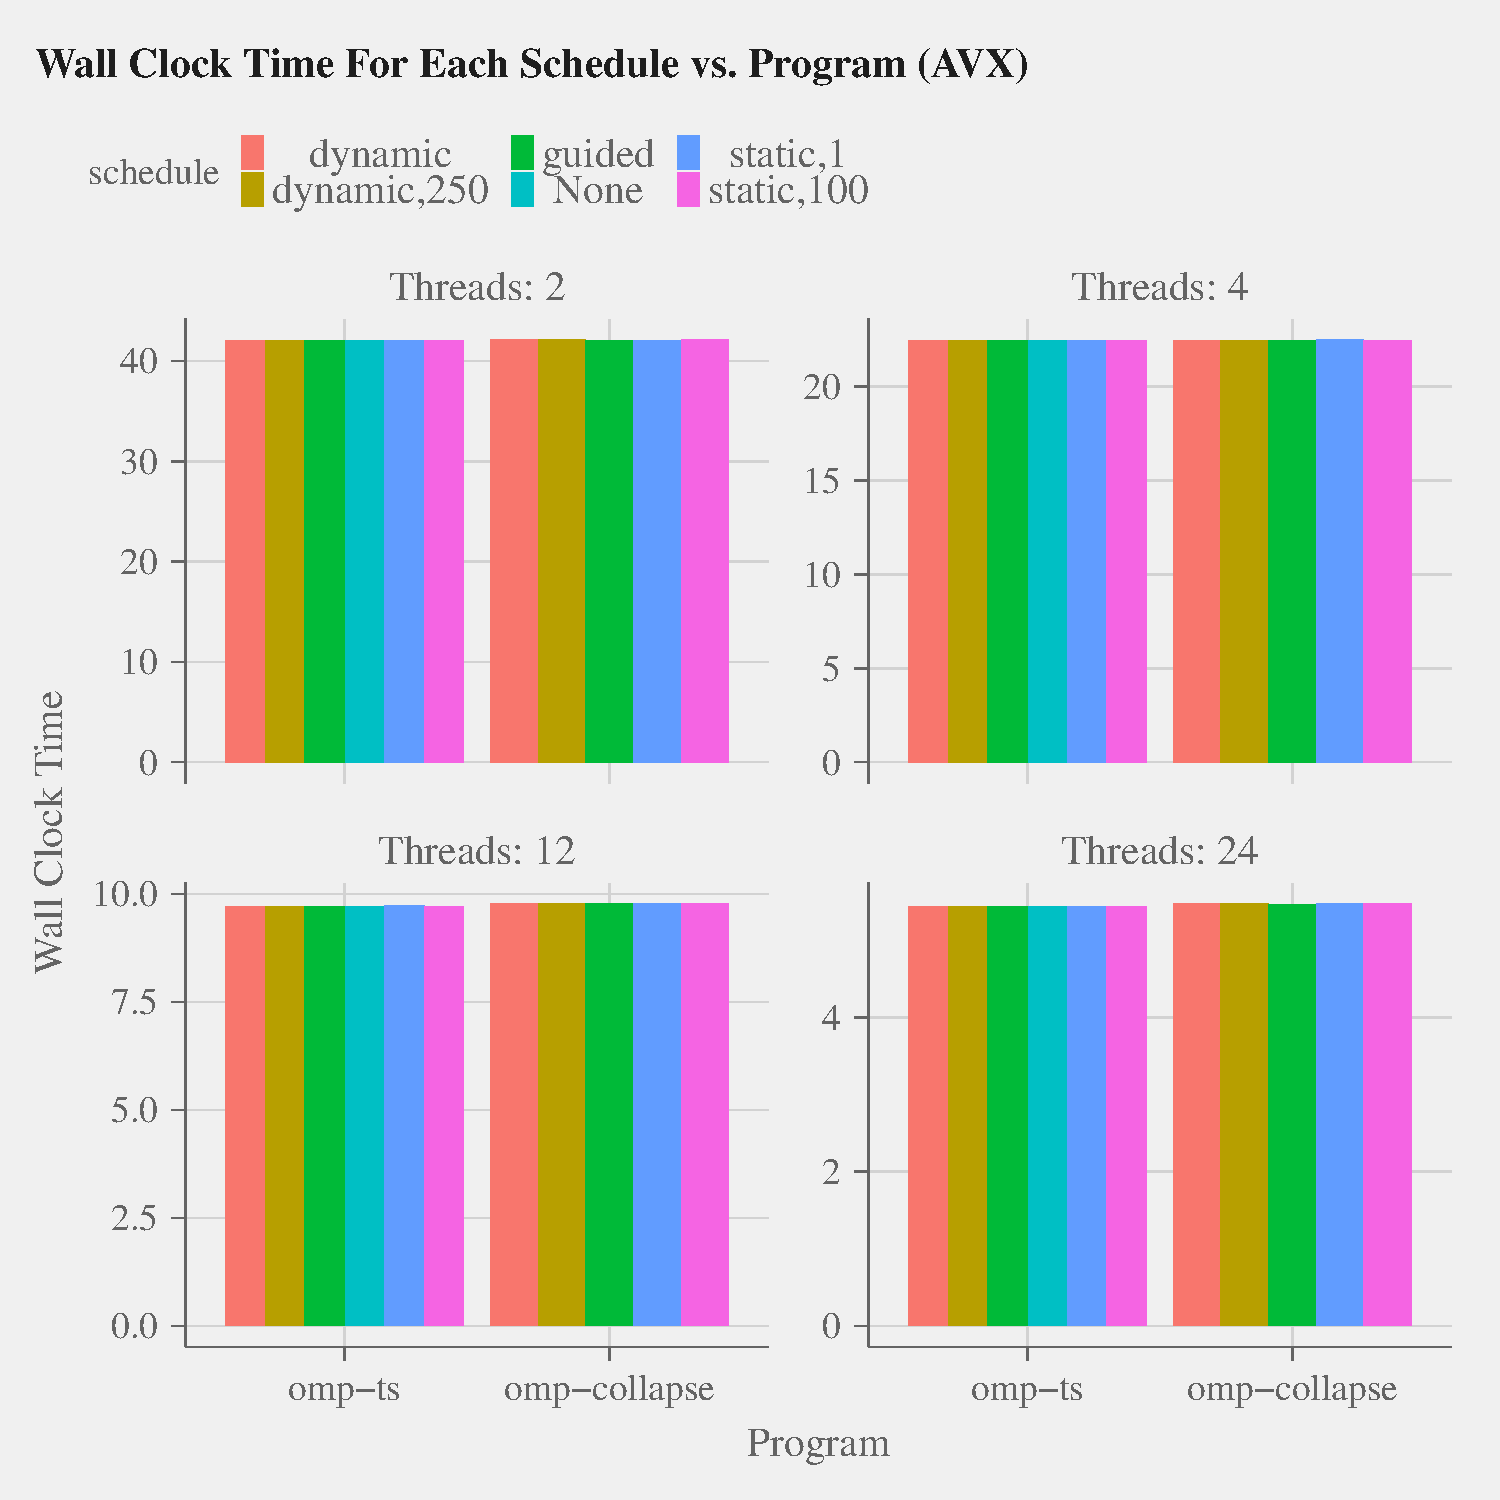
\includegraphics[width=0.9\linewidth]{q2-img.pdf} }}%
    \qquad
    \subfloat[\centering label 2]{{\includegraphics[width=0.9\linewidth]{q2-avx.pdf} }}%
    \caption{2 Figures side by side}%
    \label{fig:example}%
\end{figure}

\section{OpenMP Tasks}

\section{Parallel Random Number Generation}

\end{document}

